% Mo Jabeen Template for docs 

\documentclass[11pt]{scrartcl} % Font size

%%%%%%%%%%%%%%%%%%%%%%%%%%%%%%%%%%%%%%%%%
% Wenneker Assignment
% Structure Specification File
% Version 2.0 (12/1/2019)
%
% This template originates from:
% http://www.LaTeXTemplates.com
%
% Authors:
% Vel (vel@LaTeXTemplates.com)
% Frits Wenneker
%
% License:
% CC BY-NC-SA 3.0 (http://creativecommons.org/licenses/by-nc-sa/3.0/)
% 
%%%%%%%%%%%%%%%%%%%%%%%%%%%%%%%%%%%%%%%%%

%----------------------------------------------------------------------------------------
%	PACKAGES AND OTHER DOCUMENT CONFIGURATIONS
%----------------------------------------------------------------------------------------

\usepackage{amsmath, amsfonts, amsthm} % Math packages

\usepackage{listings} % Code listings, with syntax highlighting

\usepackage[english]{babel} % English language hyphenation

\usepackage{graphicx} % Required for inserting images
\graphicspath{{Figures/}{./}} % Specifies where to look for included images (trailing slash required)

\usepackage{booktabs} % Required for better horizontal rules in tables

\numberwithin{equation}{section} % Number equations within sections (i.e. 1.1, 1.2, 2.1, 2.2 instead of 1, 2, 3, 4)
\numberwithin{figure}{section} % Number figures within sections (i.e. 1.1, 1.2, 2.1, 2.2 instead of 1, 2, 3, 4)
\numberwithin{table}{section} % Number tables within sections (i.e. 1.1, 1.2, 2.1, 2.2 instead of 1, 2, 3, 4)

\setlength\parindent{0pt} % Removes all indentation from paragraphs

\usepackage{enumitem} % Required for list customisation
\setlist{noitemsep} % No spacing between list items

\usepackage{array}
\newcolumntype{P}[1]{>{\centering\arraybackslash}p{#1}} %Allows centering of tables

\usepackage[
backend=biber,
style=ieee,
sorting=ynt
]{biblatex}

\addbibresource{refs.bib} %Imports bibliography file

%----------------------------------------------------------------------------------------
%	DOCUMENT MARGINS
%----------------------------------------------------------------------------------------

\usepackage{geometry} % Required for adjusting page dimensions and margins

\geometry{
	paper=a4paper, % Paper size, change to letterpaper for US letter size
	top=2.5cm, % Top margin
	bottom=3cm, % Bottom margin
	left=3cm, % Left margin
	right=3cm, % Right margin
	headheight=0.75cm, % Header height
	footskip=1.5cm, % Space from the bottom margin to the baseline of the footer
	headsep=0.75cm, % Space from the top margin to the baseline of the header
	%showframe, % Uncomment to show how the type block is set on the page
}

%----------------------------------------------------------------------------------------
%	FONTS
%----------------------------------------------------------------------------------------

\usepackage[utf8]{inputenc} % Required for inputting international characters
\usepackage[T1]{fontenc} % Use 8-bit encoding

\usepackage{fourier} % Use the Adobe Utopia font for the document

%----------------------------------------------------------------------------------------
%	HEADERS AND FOOTERS
%----------------------------------------------------------------------------------------

\usepackage{scrlayer-scrpage} % Required for customising headers and footers

\ohead*{} % Right header
\ihead*{} % Left header
\chead*{} % Centre header

\ofoot*{} % Right footer
\ifoot*{} % Left footer
\cfoot*{\pagemark} % Centre footer

%----------------------------------------------------------------------------------------
%	SECTION TITLES
%----------------------------------------------------------------------------------------
 % Include the file specifying the document structure and custom commands

%----------------------------------------------------------------------------------------
%	TITLE SECTION
%----------------------------------------------------------------------------------------

\title{	
	\normalfont\normalsize
	\vspace{20pt} % Whitespace
	{\huge Database Fundamentals}\\ % The assignment title
	\vspace{12pt} % Whitespace
	\rule{\linewidth}{2pt}\\ % Thick bottom horizontal rule
}

\author{\small Mo D Jabeen} % Your name

\date{\normalsize\today} % Today's date (\today) or a custom date

\begin{document}

\maketitle % Print the title

\section{Evolution of database design}

\subsection{What has triggered the evolution in database?}

\begin{itemize}
	\item Business need to be agile, hypothesis/business models need to be tested fast and then
	decisions made if a pivot is required. Market insights should allow for quick changes to products/operations.
	\item CPU improvement is decelerating, and parallelism is increasing
\end{itemize}

\subsection{What is data intensive application?}

A data intensive application primary challenge is the use of data (storage, transformation, transmission etc)
this is primary bottle neck whereas in compute intensive apps CPU cycles is the bottle neck.

\section{Fundamental metrics}

\textbf{Reliability:} Tolerate hardware,software and human faults.\\

Fault and failure are different.

\begin{itemize}
	\item Fault: Deviates from specification
	\item Failure: Where the system stops working
\end{itemize}

Better to build fault tolerant systems that don't lead to failure. Occasionally (ie system security)
better to be fault preventive.

Worth creating faults as a testing methodology and questioning any assumptions the code bases uses to
run successfully. Systematic faults are often caused by code assumptions which are true most of the 
time. 

\subsubsection{How do you prevent human error?}

\begin{itemize}
	\item Allow fast roll backs to default configs
	\item Allow for data to be recomputed
	\item Setup good telemetry (monitoring of system health)
\end{itemize}

\textbf{Scalability:} Maintain load and performance as quantities increase.\\

\subsubsection{How do you determine the focus on when increasing scalability?}

Initial focus should be on determine the most intrinsic load parameter to the current architecture 
(ie database size, size of average reads etc).

Then question what is the effect on performance given the current resources as the load parameter is increased OR
how would the resources have to be changed.

\subsubsection{How do you measure performance?}

The most releavant performance metric should be determined (ie throughput, response time latency.) \\

This metric will most likely have a distribution even given local consistency due to external factors. The mean of this
value should generally be ignored as it does not represent an actual value experienced by the system. Instead the
median is an effective tool and the use of percentiles (50th,95th,99th etc).

\subsubsection{How to scale?}

Common knowledge is to scale on a single node before moving to a multi node setup as it is simpler. This is until it
is worth the cost of the change. \textbf{Better to focus on the ability to iterate quickly than scaling for a unknown future
load.}\\

\textbf{Maintainability:} Operability, simplicity and evolvability. (Ease of understanding).\\

The majority costs of software is upkeep not development. There are three main elements:

\begin{itemize}
	\item \textbf{Operability:} Easy to operate
	\item \textbf{Simplicity:} Easy to understand
	\item \textbf{Evolvability:} Easy to change
\end{itemize}

\subsubsection{How do you enable good operation?}

\begin{itemize}
	\item Good monitoring
	\item Standard tools
	\item Good documentation
	\item Predictable behavior
	\item Avoid single machine dependency
	\item Good default behavior
\end{itemize}

\textbf{Accidental complexity:} Arises from complexity of the implementation and is not inherent in the problem being
solved.

\section{Database Systems}

\subsection{What are some elements of a database system?}

\begin{itemize}
	\item Cache - Results of expensive operations
	\item Stream processing - Asynchronous processes messaging
	\item Batch processing - Crunch a large amount of accumulated data
	\item Message queue - Hold data for use with other processes
\end{itemize}

\subsection{Which tool should you use?}

No single tools fits all applications, instead the work should be broken into tasks
and then the most appropriate/effective tool used. 

\textit{Example: Caching - Memcached}

\section{Internal vs External}

\subsection{In code data structures}

Data structures in code should be structured and used differently to external databases. In code
data ie for OOP should be based around their use in logic. Databases can be used by multiple separate
processes whereas data structs should only be used by local code.\\

Data structs should:

\begin{itemize}
	\item Be limited in size
	\item Not generally used for concurrent programs
	\item Not tied to ACID (Atomic,consistent,isolated and durable)
	\item Fast
\end{itemize}

\section{Data Representation}

Data representation is crucial as it will directly influence how a problem is solved. The choice of method of storage is
key:

\begin{itemize}
	\item JSON
	\item XML
	\item relational db
	\item graph models
\end{itemize}

The most popular current db model is SQL, which is based on using relational databases via relational database management
systems.

NoSQL was born from:
\begin{itemize}
	\item Need for greater scalability with a large writing throughput
	\item Desire for more dynamic and expressive data modelling (schemas can be static)
\end{itemize}

\subsection{How to handle many to one relationships?}

\begin{enumerate}
	\item Ref to another table with a foreign key
	\item XML or json to have multiple entries per row
	\item Refer to a XML or JSON doc in the entry
\end{enumerate}

In relational dbs can use \textbf{joins} to combine related data, however more difficult to handle with document or NoSQL dbs.
As an apps features grows more data is collected with key links to old data increasing the \textbf{many to many relationship issue.}\\

\textit{The key issue is to solve the many to many relationship without duplication (lacking normalisation).}

\subsection{What are document databases good for ?}

The data is normally stored in one continous string, so if all the data is loaded into the app at onces, have great locality. However normally recommended to separate docs
as if any changes are needed to that cause the file size to change the entire file will be rewritten.\\

Have a very flexible schema, allowing the use of heterogenous data ie 

\begin{itemize}
	\item Each object requires a different table
	\item Data is from external sources and its format may change
\end{itemize}

Not so good at dealing with many to one or many to many relationships.

\subsection{Declarative or imperative lang?}

SQL is declarative, the compiler will decide how to implement the requirements. An imperative lang dedicates how to perform
the requirements of the code (ie the sequence the code is executed).

\subsubsection{Why is declarative useful ?}

Good at abstracting away the db implementation, allowing the RDBM to optimize without needing to changing queries. Also
great for parallel computing.

\subsubsection{How can you use SQL features with NoSQL?}

NoSQL is implementing methods to allow working easily with subsets of data ie map and reduce. The two different methods
are converging.

\section{Storage and retrieval}

\subsection{Appended files}

\subsubsection{What is the simplest method of storage ?}

Simplest most effective method is to use an append log for storage.

\subsubsection{How do you speed up retrival ?}

Without parsing through the document, retrieval is speed up by using an index.\\

\textbf{However there is a trade off, as index updating will slow down your write speed.}

\subsubsection{How does a hash index work ?}

Store all keys to the hash in memory allowing for quick looks ups. Will cause issues
if the memory size issues with a large key set. 

Works best with a small set of keys that are often changed.\\

Con: Difficult to work with range queries, as index are not stored sequentially.

\subsubsection{How do you manage the size of the append log ?}

Segment the files compress and remove any duplication. The segmented files can be
concurrently merged back.

\subsubsection{What is the standard search approach for finding a key?}

Search the most recent segment, then the next most recent etc.

\subsubsection{How are delted entries managed?}

A special message is appended into the log, which is used to ignore the chosen entry
at the next merge.

\subsection{LSM / SS Tables}

\subsubsection{What if you sort the key value pairs ?}

In hash indexes the key value pairs are stored sequentially. In a Sorted String table (SS Table)
the key value pairs are sorted by key. Can then make assumptions about the location of a value,
due to the ref values and the expected order. Can take these segments between ref values and 
compress them for better bandwidth.

\subsubsection{How is a LSM tree created ?}

\begin{enumerate}
	\item Write to in memory structured tree, by key.
	\item When big enough store data in a SSTable sorted by key
	\item Read data by first checking the mem table then the SSTables in disk
	\item Merge and compress segments on disk in the background
\end{enumerate}

\subsubsection{What are issues with LSM trees?}

When writing the memtable to disk a cash would cause lost data, so append logs are used to store
data in the memtable deleted when memtable stored as SStable. 

\subsubsection{How do you optimize finding a key?}

Use \textbf{Bloom filters} to quick check if a key is in a segment.

\subsection{B trees}

\subsubsection{What is the most standard index implementation?}

B trees are the most widely used and standard index implementation. They use fixed size blocks called pages. LSM are
appended B trees changed in place. Fixed size implementation matches how storage is done in hardware.

\subsubsection{How are B trees built?}

Pages are linked to each other, some pages refer to child pages via a ref key value and the boundaries between the
given references show which which child page will hold the key being searched for.

\begin{figure}[h] % [h] forces the figure to be output where it is defined in the code (it suppresses floating)
	\centering
	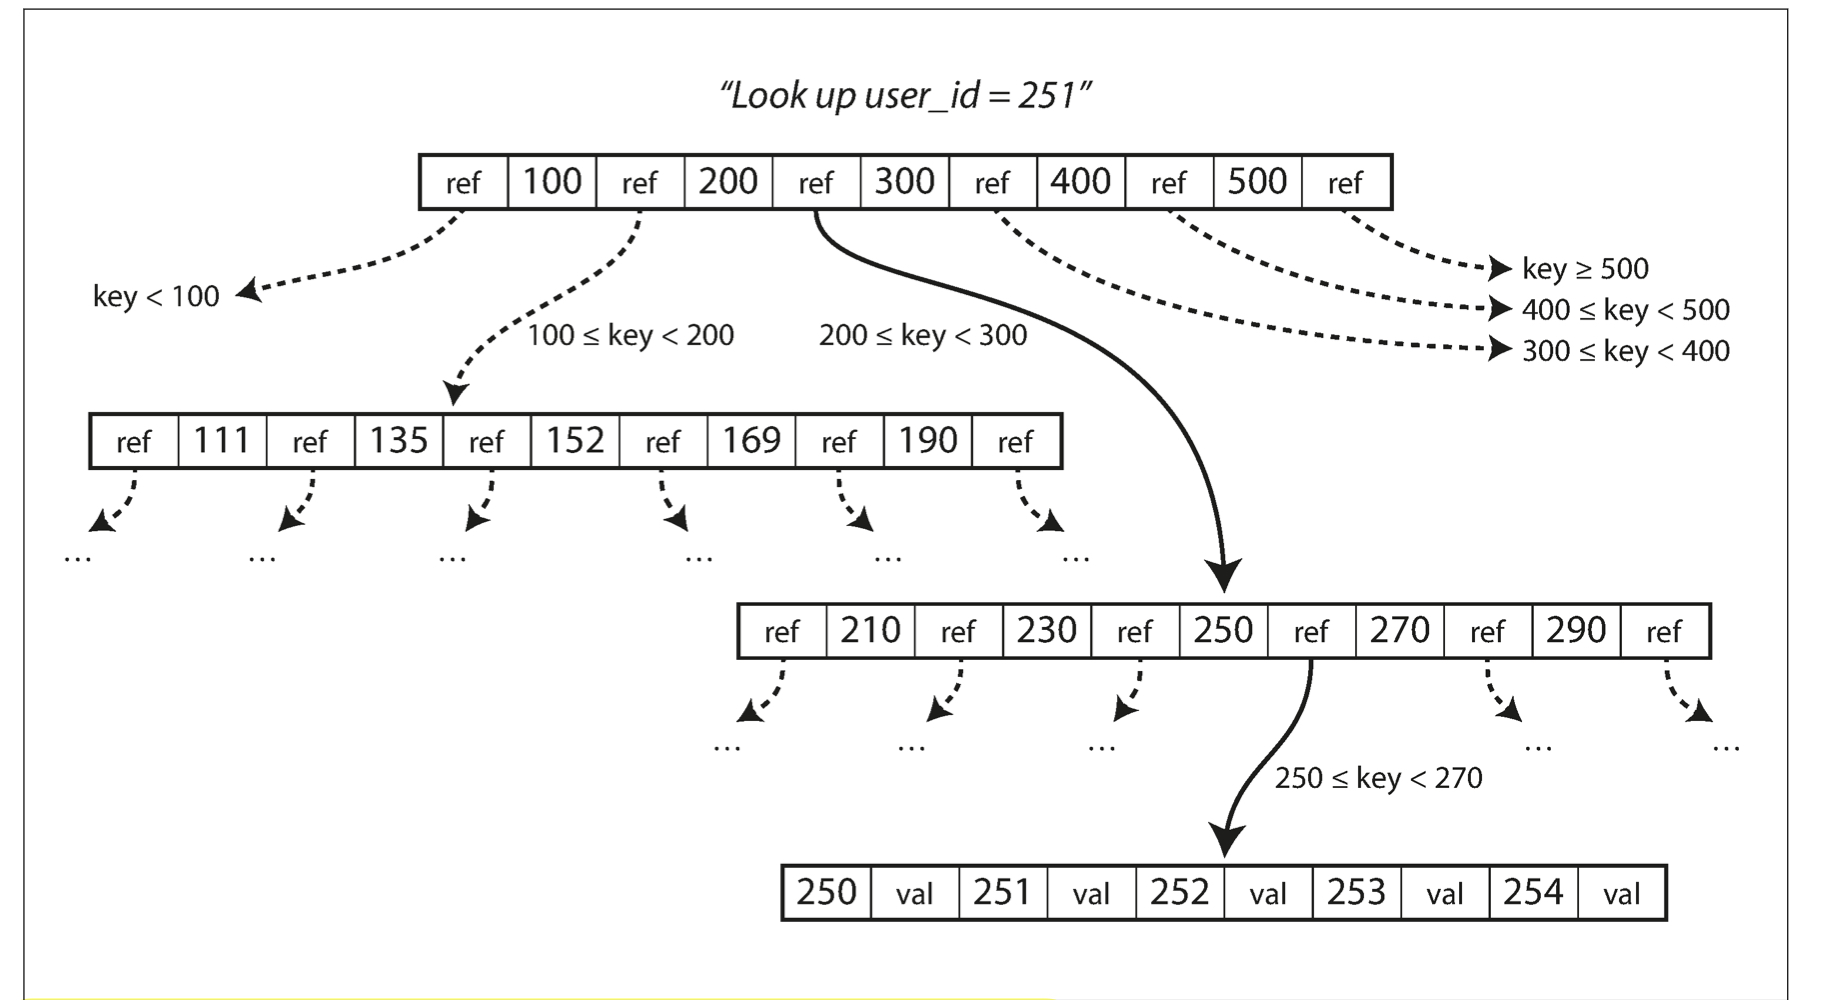
\includegraphics[width=\columnwidth]{B trees construction.jpeg} % Example image
	\caption{B trees page construction}
\end{figure}

Some pages will have the actual key and its value for indexing, these are called leaf pages. The number
of refs in a page is called branching factor. 

If a page does not have enough space for a new key, its split into two and the references are updated.

A four level tree with 4kB pages and a branching factor of 500 can hold 256 TB of data. The actual data
stored is structured into the tree.

\subsubsection{What are the issues with B trees ?}

When splitting a tree and updating the references is there is a crash in between can create corrupt data.
So write ahead logs are used, a file that appends changes before they are executed.

They also need to be careful when dealing with concurrency due to the required in place writes. So use
latches (light weight locks).

\subsubsection{How can B tree performance be improved?}

Write a new modified page and change the reference to it, this will be more performance effective than
modifying a page and keeping a write ahead log.

\subsubsection{What is better LSM or B trees ?}

Rule of thumb:

\begin{itemize}
	\item LSM has better write throughput
	\item B trees have better reads
\end{itemize}

However many optimizations to B trees to improve its write throughput.

\section{Transactional vs Analytical Data}

\subsubsection{What are Transaction and Analytical processes?}

Transaction process track every day writes with updates happening often. Allows for low latency
small reads and writes. \textbf{OLTP - Online Transaction Processing}. 

OLTP data is crucial for business so queries and bandwidth is tightly controlled.\\

Analytical processes are large data amounts queried and uses for analysis. Generally these are instead
stored in a date warehouse, which uses very different patterns for indexing (Not B or LSM trees). 
\textbf{OLAP - Online Analytical Processing}.

\subsubsection{How are data warehouses created ?}

The data warehouse includes copies of the data in the OLTP data that has been extracted, transferred and
then dumped into the database. \textbf{ETL - Extract Load and Transform}

They most commonly use relational databases ie sql.

\subsubsection{What is star and snowflake schema ?}

\textbf{Star schema: One main fact table then many dimension tables ie product SKU, date ID etc}\\
\textbf{Snowflake schema: Has many layers of dimensions.}

\subsection{What is column storage ?}

Instead of storing all values from each row together, instead store all values from each col.

Therefore queries only need to query and parse the values used in the query. This is bad for OLTP
as you will need to look and edit many files/tables for every transaction.

\subsubsection{How do you compress column storage ?}

Bitmap encoding is a form of compression, where one bitmap is created for every distinct value
and one for each row. If that row contains that value the bit is 1 or 0 if it does not.

Good for smaller number of distinct values used. Can be good for CPU cycles too as compressed data
can be perform bit operations directly.\\

Sorted cols can be used for faster queries ie sort by most queried.\textbf{ALl columns must use
the same order for all files so a row can be reconstructed.}\\

Can also create summary "materlized view" tables allowing for quick queries when comparing two
dimensions, such as sum.\\

Colum storage uses a similar concept to LSM trees for storage, hold in memory then written to disk.
B trees are very hard as doing in places changes over many files will be very difficult.

\section{Encoding and Evolvability}

Changes to the schema caused by new features and data. Old and new code should be able to deal with
these changes. Should also allow staged rollouts for better evolvability with small frequent changes.

\subsubsection{What is the difference between in code data and data sent over the network ?}

In code the data is stored in the programs structures, which are optimized to work with the CPU
and use a pointer to access. \\

Over a network you need a self contained sequence of bytes ie JSON sent using some type of protocol
ie HTTP.

\subsubsection{How do you convert from memory to network data ?}

Encoding, marshalling and serlization are terms for changing program data to byte sequences.The
reverse is decoding, unmarshalling and deserilization.

\subsubsection{What is the issue with the libarires used by langs to encode/decode?}

\begin{itemize}
	\item Program specific
	\item Allows arbitrary classes to be instantiated (which is a security issue)
	\item Bad performance/compatibility
\end{itemize}

These should be only used for a small period of time and small issues.

\subsubsection{What are the types of Encodings?}

The most standard and popular are JSON and XML (which is considered too complex).\\

Binary encoding are more space efficient, however are not in a human readable format.When TB of data
is being sent this will matter. Apache thrift, protocol buffer and avaro (particularly flexible schema) are examples of binary encodings.
They also gave a much simpler and less strict schemas rules giving better evolvability.

\subsection{Modes of data flow}

\subsubsection{What are potential issues with using a database as a dataflow ?}

Will often have many processes accessing the db at any given time, its important that different
version of code work with the database. New data for a col should work with old and new code.\\

Forward compatibility is particularly important, there is a need to be careful of lost data in old code
collecting data from the db converting it to an object then converting back to be placed into the db!!!\\

Migrating to new schemas is expensive so instead old data is left and new data is fitted into the db,
ie use a default null val to a new col.

\subsubsection{How is data sent over a network?}

Severs that expose data request via an API are called services. APIs use an agreed standard set of
protocols ie HTTP,URL, TLS etc. Web apps uses services and a JavaScript app using XMLHTTPRequest to become
a HTTP client is known Ajax.\\

Services are similar to a database allowing input and output of data, however they are very 
restricted by the business logic giving encapsulation.

\subsubsection{What are the HTTP API methods ?}

The two most popular are REST and SOAP. REST is a philosophy based around the tools of HTTP. SOAP
is XML based and is trying to be HTTP independent, uses a bunch of features from the web service
framework. Also uses an XML lang which can be good for statically typed languages.\\

RESTful APIs are more popular and use Swagger as a definition format.

\subsection{What about RPCs ?}

Remote procedure calls (RPCs) are formed on the idea of making network calls feel like calling a
local function. Which is called location based transparency.

\subsubsection{What is bad about RPCs?}

Local function and remote functions are not the same:

\begin{itemize}
	\item Network may return no result ie timeout
	\item Retrying may make a process run many times in a service
	\item Network calls will differ in latency
	\item Program data sent as encoded bytes can be problematic
\end{itemize}

\subsubsection{Examples of RPCs ?}

\begin{itemize}
	\item gRPC uses protocol buffer
	\item Fingle uses Thrift
	\item Rest.li uses JSON over HTTP
\end{itemize}

Binary encoded RPC have better performance than generic methods ie JSON using REST.

\subsubsection{What are message brokers ?}

The middle men used a data queue to make messaging safer and simpler.

Send message to queue or topic, message is sent from topic to subscriber or consumer.

\subsection{What are actor models used for ?}

Used for concurrency, an actor is an entity that sends messages to each other. As only one message
is dealt with the worry of threads is gone.

%----------------------------------------------------------------------------------------
%	FIGURE EXAMPLE
%----------------------------------------------------------------------------------------

% \begin{figure}[h] % [h] forces the figure to be output where it is defined in the code (it suppresses floating)
% 	\centering
% 	\includegraphics[width=0.5\columnwidth]{IMAGE_NAME.jpg} % Example image
% 	\caption{European swallow.}
% \end{figure}

%----------------------------------------------------------------------------------------
% MATH EXAMPLES
%----------------------------------------------------------------------------------------

% \begin{align} 
% 	\label{eq:bayes}
% 	\begin{split}
% 		P(A|B) = \frac{P(B|A)P(A)}{P(B)}
% 	\end{split}					
% \end{align}

%----------------------------------------------------------------------------------------
%	LIST EXAMPLES
%----------------------------------------------------------------------------------------

% \begin{itemize}
% 	\item First item in a list 
% 		\begin{itemize}
% 		\item First item in a list 
% 			\begin{itemize}
% 			\item First item in a list 
% 			\item Second item in a list 
% 			\end{itemize}
% 		\item Second item in a list 
% 		\end{itemize}
% 	\item Second item in a list 
% \end{itemize}

%------------------------------------------------

% \subsection{Numbered List}

% \begin{enumerate}
% 	\item First item in a list 
% 	\item Second item in a list 
% 	\item Third item in a list
% \end{enumerate}

%----------------------------------------------------------------------------------------
%	TABLE EXAMPLE
%----------------------------------------------------------------------------------------

% \section{Interpreting a Table}

% \begin{table}[h] % [h] forces the table to be output where it is defined in the code (it suppresses floating)
% 	\centering % Centre the table
% 	\begin{tabular}{l l l}
% 		\toprule
% 		\textit{Per 50g} & \textbf{Pork} & \textbf{Soy} \\
% 		\midrule
% 		Energy & 760kJ & 538kJ\\
% 		Protein & 7.0g & 9.3g\\
% 		\bottomrule
% 	\end{tabular}
% 	\caption{Sausage nutrition.}
% \end{table}

%----------------------------------------------------------------------------------------
%	CODE LISTING EXAMPLE
%----------------------------------------------------------------------------------------

% \begin{lstlisting}[
% 	caption= Macro definition, % Caption above the listing
% 	language=python, % Use Julia functions/syntax highlighting
% 	frame=single, % Frame around the code listing
% 	showstringspaces=false, % Don't put marks in string spaces
% 	numbers=left, % Line numbers on left
% 	numberstyle=\large, % Line numbers styling
% 	]

% 	CODE

% \end{lstlisting}

%----------------------------------------------------------------------------------------
%	CODE LISTING FILE EXAMPLE
%----------------------------------------------------------------------------------------

% \lstinputlisting[
% 	caption=Luftballons Perl Script., % Caption above the listing
% 	label=lst:luftballons, % Label for referencing this listing
% 	language=Perl, % Use Perl functions/syntax highlighting
% 	frame=single, % Frame around the code listing
% 	showstringspaces=false, % Don't put marks in string spaces
% 	numbers=left, % Line numbers on left
% 	numberstyle=\tiny, % Line numbers styling
% 	]{luftballons.pl}

%------------------------------------------------

\end{document}